%----------------------------------------------------------------------------------
% Exemplo do uso da classe tcc.cls. Veja o arquivo .cls
% para mais detalhes e instruções.
%----------------------------------------------------------------------------------
\chapter{Fundamentação Teórica}\label{chap2:fund_teo}
    \section{USV}\label{subchap2:USV}
        \textit{"Unmanned Surface Vehicle"}, ou veículo de superfície não tripulado, é caracterizado por realizar atividades navais de forma autônoma, ou controlado remotamente, sem a presença de tripulação.~\cite{LIU201671} Tais caracteríscticas também enquadram um USV na categoria de um robô.~\cite{JUR2020}
        
        De acordo com [Liu], um USV pode ter as mais variadas aparências e funcionalidades, porém os seguintes componentes básicos devem sempre compor um USV:~\cite{LIU201671}
        
        \begin{enumerate}
            \item Casco e estruturas mecânicas auxiliares
            \item Sistema de Propulsão
            \item Sistema GNC (\textit{"Guidance Navigation and Control"})
            \item Sistema de Comunicação
            \item Equipamento de Coleta de Dados
            \item Estação de Solo
        \end{enumerate}
        
        Dentre os elementos listados o sistema GNC é fundamental para tornar automatizar um USV, pois é ele quem controlará o sistema do USV como um todo. Sua função consiste coletar informações a respeito do USV e seu entorno (\textit{"Navigation"}), determinar o melhor caminho a seguir com base nos dados coletados (\textit{Guidance}) e executar as ações necessárias para seguir a melhor rota encontrada (\textit{"Control"}).  ~\cite{LIU201671} ~\cite{JUR2020} Com isso, é responsabilidade do GNC executar todas as etapas necessárias para a prevenção de colisão~\cite{HUANG2020451}, que serão abordadas na sessão ~\ref{subchap2:prev_col}. 
        
        \begin{figure}
            \centering
            \includegraphics{}
            \caption{Caption}
            \label{fig:gnc_system}
        \end{figure}
    
    
    \section{Prevenção de Colisão}\label{subchap2:prev_col}
        Uma tarefa primordial quando se trata de navegação é evitar que a embarcação colida com algum obstáculo. Porém, é alto o número de acidentes com embarcações envolvendo colisões. Além disso, diversas investigações apontam que a principal causa desses acidentes é o fator humano.~\cite{HUANG2020451}
        
        Frente ao alto número de ocorrencias dessa natureza, pesquisadores vem estudando meios de evitar tais acidentes. [Huang] afirma que atualmente há duas frentes na tecnologia de prevenção de colisão: (1) assitência à tripulação e (2) eliminação de fatores humanos. Sendo esta última a perspectiva abordada neste trabalho dado que o componente físico de implementação é um USV.~\cite{HUANG2020451}
        
        Huang (2020, p.2) define prevenção de colisão como:
        \begin{directcite}
            \textit{"Prevenção de colisão é o processo em que um navio desvia de sua trajetória planejada para evitar contato físico indesejado em um certo tempo futuro"}
        \end{directcite}
        
        Com isso, [Huang] separa o processo de prevenção de colisão nas etapas de "detecção de conflito", que determina se o navio está em risco de colisão ou não, e "resolução de conflito", que define quais ações devem ser tomadas pelo navio para evitar a colisão. Em um USV, tais atividades são atribuidas ao módulo de \textit{"Guidance"} do sistema GNC.~\cite{HUANG2020451}
        
        Na Figura~\ref{fig:col_avoid_info_flow} é possível observar o fluxo de informação por entre os módulos que compõe um sistema de evasão de colisão. Em suma, o módulo \textit{"Observer"} coleta informações através de seus sensores e câmeras; \textit{"Motion Prediction"} faz uso dos dados coletados pelo módulo anterior para estimar as futuras posições do OS e do TS; \textit{"Conflict Detection"} ineterpreta as informações fornecidas pelos módulos anteriores para verificar se há o risco de colisão; havendo risco de colisão, o módulo \textit{"Conflict Resolution"} é acionado para determinar as ações necessárias para evadir da situação de risco; o módulo \textit{"Actuator"} executa as ações definidas pelos módulos anteriores.~\cite{HUANG2020451}
        
        \begin{figure}
            \centering
            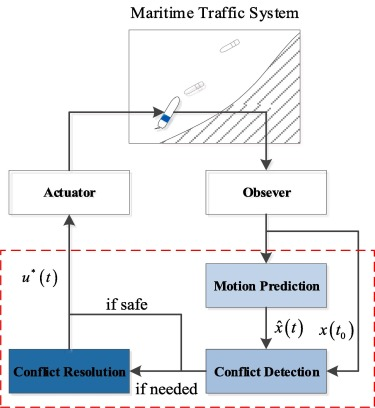
\includegraphics{fig/information_flow.png}
            \caption{Fluxo de informação ~\cite{HUANG2020451}}
            \label{fig:col_avoid_info_flow}
        \end{figure}
        
        Os módulos envoltos ao pontilhado vermelho na Figura~\ref{fig:information_flow} formam o sistema de evasão de colisão. 
        
    \subsection{}